\usetikzlibrary{arrows.meta,calc}
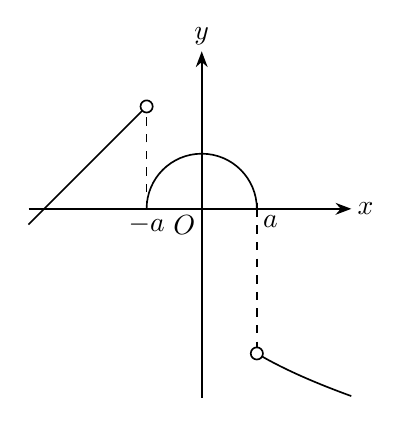
\begin{tikzpicture}[x=1cm,y=1cm,line width=.6pt,>=Stealth,font=\normalsize]
\draw[->] (-2.2,0)--(1.9,0) node[right,inner sep=0pt,xshift=2pt] {$x$};
\draw[->] (0,-2.4)--(0,2.0) node[above,inner sep=0pt,yshift=2pt] {$y$};
\node[below left,inner sep=0pt,xshift=-2pt,yshift=-2pt] at (0,0) {$O$};
\draw[line width=.6pt] (-0.7,0)--(-0.7,0.07);
\draw[line width=.6pt] (0.7,0)--(0.7,0.07);
\node[below,inner sep=0pt,yshift=-2pt] at (-0.7,0) {$-a$};
\node[below right,inner sep=0pt,xshift=2pt,yshift=-2pt] at (0.7,0) {$a$};
% upper semicircle radius a (representative 0.7)
\draw (-0.7,0) arc[start angle=180,end angle=0,radius=0.7];
% ray y=x+2
\draw (-2.2,-0.2)--(-0.7,1.3);
% curve y=-sqrt(x)-1
\draw[domain=0.7:1.9,samples=60] plot (\x,{-sqrt(\x)-1});
% dashed droplines
\draw[dashed] (-0.7,0)--(-0.7,1.22);
\draw[dashed] (0.7,0)--(0.7,-1.7567);
% open endpoints
\draw[fill=white] (-0.7,1.3) circle (2.2pt);
\draw[fill=white] (0.7,-1.83666003) circle (2.2pt);
\end{tikzpicture}
